% Modified from https://github.com/PetarV-/TikZ/blob/master/Graph%20convolution/graph_convolution.tex

\documentclass[crop, tikz]{standalone}
\usepackage{tikz}

\usetikzlibrary{arrows,shapes}

\definecolor{mygreen}{rgb}{0,0.6,0}

\pgfdeclarelayer{background}
\pgfsetlayers{background,main}

\tikzstyle{vertex}=[circle,fill=black!25,minimum size=20pt,inner sep=0pt]
\tikzstyle{selected vertex} = [vertex, fill=red!24]
\tikzstyle{select vertex} = [vertex, fill=blue!24]
\tikzstyle{selectx vertex} = [vertex, fill=green!24]
\tikzstyle{edge} = [draw,thick,-]
\tikzstyle{selected edge} = [draw,line width=5pt,-,red!50]

\begin{document}

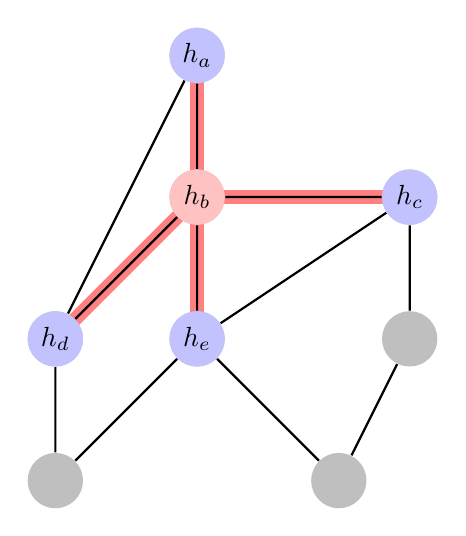
\begin{tikzpicture}[scale=1.8, auto,swap]
    \foreach \pos/\name in {{(2,2)/a}, {(2,1)/b}, {(3.5,1)/c},
                            {(1,0)/d}, {(2,0)/e}, {(1,-1)/f}, {(3,-1)/g}, {(3.5,0)/h}}
        \node[vertex] (\name) at \pos {};
        
    \foreach \source/ \dest /\weight in {b/a/7, c/b/8, d/a/5, d/b/9,
                                         e/b/7, e/c/5, c/h/7,
                                         f/d/6, f/e/8, g/h/9,
                                         g/e/9}
        \path[edge] (\source) -- (\dest);
         
    \foreach \vertex / \fr in {b/4}
        \path node[selected vertex] at (\vertex) {$h_b$};
    \foreach \vertex / \fr in {a/4, c/4, d/4, e/5}
        \path node[select vertex] at (\vertex) {$h_{\vertex}$};
    \begin{pgfonlayer}{background}
        \foreach \source / \dest in {b/c,d/b,a/b,b/e}
            \path[selected edge] (\source.center) -- (\dest.center);
    \end{pgfonlayer}

\end{tikzpicture}

\end{document}